\\
The objective is to design a two level three phase inverter to drive the go-carts PMSM motor. This basically consist of six switches and some capacitance on the DC-link. On figure \ref{fig:Sketch_PowerBoard} a simple model of the Power board is shown.

    \begin{figure}[H]
		\centering
		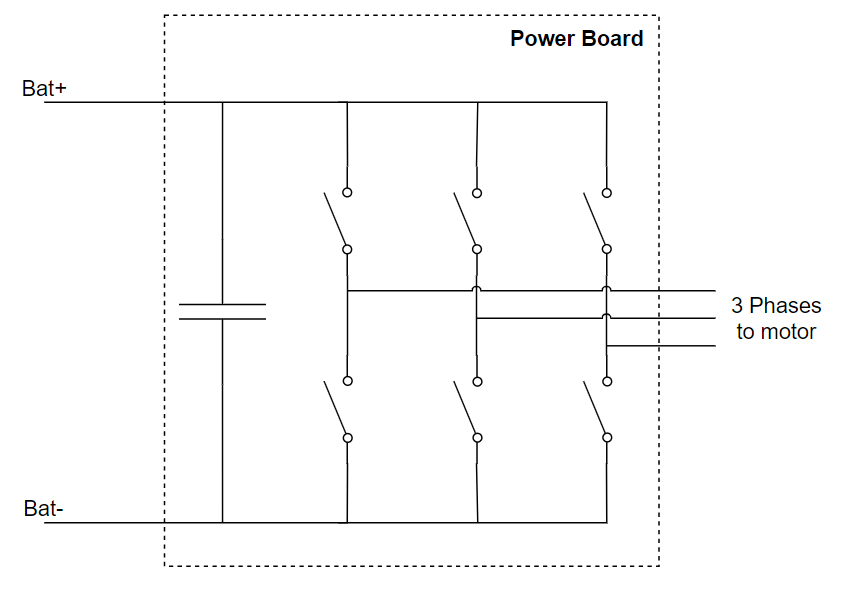
\includegraphics[width=0.7\textwidth]{pictures/hardware/Power_Board/Sketch_of_powerBoard.PNG}
		\caption{Sketch of the Power Board}
		\label{fig:Sketch_PowerBoard}
	\end{figure} 
	
This means that there have to be selected a switch component. The switch component has a great impact on the inverter design, due to that it is a big source of losses in the inverter. It is therefore important to choose a good transistor for switching. Besides the switch component, there has to be selected a type PCB board for the Power board.

\subsubsection{Switching frequency} \label{switching_frequency}
When deciding a switching frequency for the inverters, the rotation frequency of the motor and the thus the frequency of the electrical field.
It is known form the Data sheet of the motor, that the maximum rotation speed of the motor is $5000 rpm$ and it has 8 poles equal to 4 pole pairs. From this the maximum frequency of the electrical field be determined.

\begin{equation}
    f = \frac{N \cdot P}{60}
    \label{eq:max_frequency}
\end{equation}

Where $N$ is the rotational speed in $rpm$ and $P$ is the number of pole pairs in the motor.
From equation \ref{eq:max_frequency} the maximum frequency of the electrical field is $333.3 Hz$.
It is desired to have between 10 and 20 switch periods per period of the electrical field. 20 switch periods per electrical field period results in a switching frequency of $6666 Hz$. It is not necessary to switch faster than the $6666 Hz$, but it is decided to use a switching frequency of $10 kHz$. This is done to make the use of smaller capacitors possible and because already so low frequency it is not a problem to increase it a bit.
It is decided not to increase the switching frequency to more than $10 kHz$ to reducing the switching losses.


\subsubsection{PCB selection}
Two types of PCB's has been considered, a ordinary multi-layer PCB and a single-layer aluminum PCB. There is of course pros and cons for both options. With the ordinary PCB there is better opportunities for conducting the heat away from the switch components. On the other hand it is not possible to use SMD components, due to the heat can not be transferred away from the components. The SMD components can result in a better and more compact layout. This is due to the SMD components is smaller and is available with multiple source legs, which minimize the common source for the switch components. The Use of SMD components will be possible with the aluminum PCB. Due to that the SMD components have a smaller area and the heat has the transferred through the aluminum PCB, the cooling of the components is a harder task. With the aluminum PCB it is not possible to use through hole components, which can have some cons when it comes to the mounting of the large capacitors for the DC-link. 

The ordinary PCB has also the benefit, that is has multiple layers. This could make it easier to layout a good power board. On the other hand, due to the budget, it will not be possible to get a PCB with much more than 2 layers anyways, maybe 4 layers. It is of course better than the single layer on the aluminum PCB. It is possible to get the aluminum PCB with two layers, but it will result in a  too high thermal resistance and price.

Based on these considerations it is chosen to use the aluminum PCB, because the benefits of the SMD components is weighted higher than the cons.


\subsubsection{Transistor selection}
The selection of transistors is a very important aspect of the design of the inverter. This due to that the transistors has great affect on the power loss in the system and thus the heat dissipation which set the limits of the design.  
Transistor selected is made from a couple of aspects. first of all the needed ratings necessary for the system. The Drain to Source current has to be rated for $300 A$ if no parallel devices is used. It is chosen that it has to have a rated Drain to Source voltage of $100 V$. This is due to the battery in the go-kart has a maximum voltage of $57.6$ plus some safety margin for voltage spikes. The maximum battery voltage is found based on the cell voltage of a $LiFePO_4$: $3.6 V$, multiplied with the number of cells, which is 16. The transistor has to have a fall time of less than $250ns$ and rise time of less than $50ns$. Besides that the transistor has to have a as low as possible on-resistance, to minimize conduction losses, which is very significance when conducting a current of $300A$.

The Transistor with these specifications and the lowest possible Drain-Source on resistance, to a affordable price, was a MOSFET. The MOSFET have the benefit of having a low current needed for turn on, the ability to handle high current needed for the motor and fast enough for the switching frequency. Since price is everything, when it comes to choice of components, then some sort of compromise will be made \\

The MOSFET chosen is an Infineon "IPB017N10N5". Some of the important specifications is listed in the table below.
\begin{center}
 \begin{tabular}{|c|c|c|} 
 \hline
 Parameters & Value & Unit \\
 \hline
 $V_{DS}$ & 100 & V \\  
 \hline
 $R_{DS-ON}$ & 1.7 & $m\Omega$ \\
 \hline
 $I_D$ & 273 & A \\
 \hline
 $Q_G$ (0-10V) & 168 & nC \\
 \hline
 $Q_{GD}$ & 34 & nC \\
 \hline
 $Q_{GS}$ & 53 & nC \\
 \hline
 $Q_{sw}$ & 51 & nC \\
 \hline
 Rise time & 23 & ns \\
 \hline
 Fall time & 27 & ns \\
 \hline
\end{tabular}
\end{center}

When looking at the parameters, a couple of things need to be considered. From the top it can be seen that the Drain-Source voltage is $100 V$, so it is able to handle the kart's battery voltage. Next the  [$I_D$] is not $300 A$ or above, which leads to a design choice of having two or more in parallel. Having more transistors in parallel has the benefit of splits the current up between them, lowering the conduction power loss. Having lower power loss decreases the amount of heat generated, which leads to less risk of overheating. The gate charge is the amount of charge that needs to be delivered to the gate from the driver, in order to turn the transistor on. This parameter needs to be as low as possible same as the Drain-Source resistance, but normally with a low resistance comes higher gate charge and vise versa. In this case is it more important that the Drain-Source on resistance is low rather than the Gate charge is low. This is the case because speed of the turning on and off of the MOSFET is reduced anyway. Besides that the increased driver power losses will not be as significant compared to the increased power losses in a MOSFET with higher Drain-Source on resistance.\\ 


\subsubsection{Power and heat dissipation in the transistors}
There are two types of power losses in the transistors. One is conduction losses, which is caused by the intern resistance in MOSFET between the Drain and the Source, when the MOSFET is conducting. The other one is switching losses, which is caused then the MOSFETs is turning on and off. Based on the power loss calculations the expected heat increase of the MOSFETs can be estimated, which will be used to decide how many MOSFETs in parallel is needed.

\paragraph{Conduction loss}
When a MOSFET is conducting there will be a power dissipation due to the intern Drain-Source on resistance in the MOSFET. Thus the conduction power loss in the MOSFETs is calculated in the same way as the power loss in a resistor. Equation \ref{eq:ConductionLossMOSFET} describes the conduction power loss for one MOSFET, $P_{con/MOSFET}$.

    \begin{equation}
        P_{con/MOSFET} = \bigg( \frac{I}{N \cdot 2} \bigg) ^2 \cdot R_{DSon}
        \label{eq:ConductionLossMOSFET}
    \end{equation}

$I$ is the peak current, $N$ is the number of transistors in parallel per switch, and $R_{DSon}$ is the Drain-Source on resistance of the MOSFET.
The peak current is divided by the number of transistors in parallel, to get the current in one MOSFET. Because the current is sinusoidal and the average duty cycle of the PWM over a period is $50 \% $, it is also divided by two to get the current one transistor is conducting.

To calculate the conduction power loss for all the transistors, it is then multiplied with the number of parallel MOSFETs per switch, two for taking both the high and low side into account, and the number of legs in the inverter, which is three.

    \begin{equation}
        P_{con} = \bigg( \frac{I}{N \cdot \sqrt{2}} \bigg) ^2 \cdot R_{DSon} \cdot N \cdot 2 \cdot 3
        \label{eq:ConductionLossTot}
    \end{equation}

On figure \ref{fig:ConductionLoss} the relationship between conduction power loss per MOSFET, equation \ref{eq:ConductionLossMOSFET}, and for all the MOSFETs, equation \ref{eq:ConductionLossTot}, is plotted as a function of the number of MOSFETs in parallel. 

    \begin{figure}[H]
		\centering
		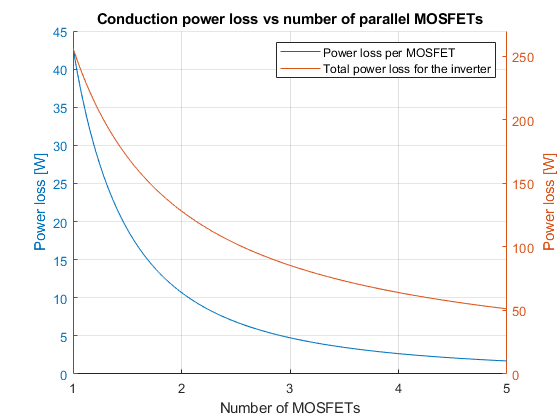
\includegraphics[width=0.8\textwidth]{pictures/hardware/Power_Board/Conduction_loss.png}
		\caption{Conduction power loss versus the number of parallel transistors in parallel per switch}
		\label{fig:ConductionLoss}
	\end{figure} 

\paragraph{Switching loss}
The other cause of power loss in the MOSFETs is the switching power loss. The switching power losses is caused by the period, when switching, where both the voltage over and the current through the MOSFET is not zero. This is called hard switching. Soft switching is when the MOSFET switching on or off without the voltage and current overlaps. This will not cost any power loss. This is illustrated on figure \ref{fig:HardSoftSwitch}.

    \begin{figure}[H]
		\centering
		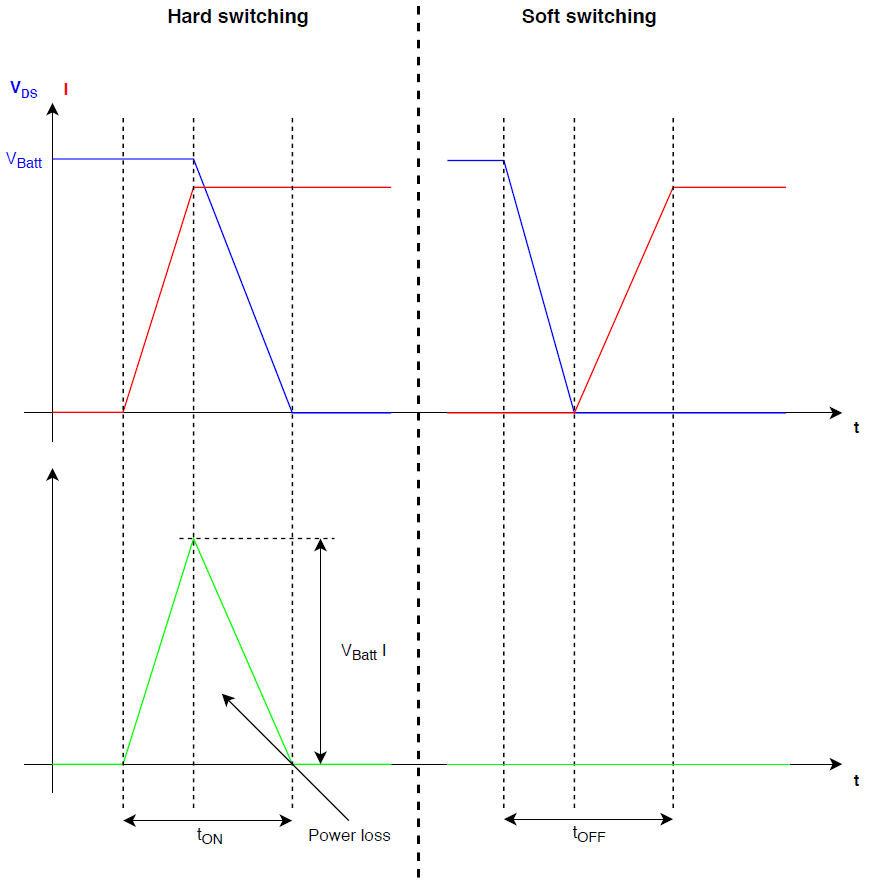
\includegraphics[width=0.8\textwidth]{pictures/hardware/Power_Board/Hard_soft_switching.PNG}
		\caption{Illustration of hard and soft switching of MOSFET}
		\label{fig:HardSoftSwitch}
	\end{figure} 

When running the motor, the motor current has a positive and a negative half cycle. During the positive half period the current going into the motor, and in the negative half period the current going from the motor into the inverter. In the positive half period the low-side switch gets soft turned on and the high-side switch gets hard turned on. Opposite in the negative half period the low-side switch is hard turned on and the high-side switch is soft turned on. This means One transistor will only hard switch $50 \%$ of the time.

The switching power is calculated as the area under the green line on figure \ref{fig:HardSoftSwitch} multiplied with the switching frequency. This is multiplied with a half because the switches is only hard switched $$ 

    \begin{equation}
        P_{sw/MOSFET} = 0.5 \cdot 0.5 \cdot V_{batt} \cdot \frac{I}{N} \cdot (t_{on}+t_{off}) \cdot f_{sw}
    \end{equation}



